\section{Application Profiling}
\label{sec:Application_Profiling}
After conducting some initial scaling experiments on the 'closest vector problem' algorithm, it became evident that scalability is an issue. Therefore, it was decided to profile the application in the search for bottlenecks and their causes. The Intel\textregistered Parallel Studio XE performance analysis tool suite was used to profile the application to gain an overview of the performance and inspect any issues in greater detail.

The profiling results shown in this section compare the performance of the application before and after applying optimisations to the \textit{nCU} gate routine discussed in Section~\ref{sec:optimisations}. Note that the \textit{nCU} optimisations did not produce the correct results, but are of a similar type and number of gates as the expected correct implementation. Thus, the comparisons provided in this section are meaningful and represent the expected optimised \textit{nCU} implementation that yields the correct results.

A number of scripts were created to launch and run each profiling tool due to the different environments required for each tool. Note, the profiling with hardware counters enabled on Kay was limited to using a maximum of four nodes since they are the only nodes with the appropriate permissions for hardware counters. A small number of processes was used to reduce the quantity of data collected.

The profiling experiments listed below were carried out using an allocation of $2$ nodes, each with $2$ processes running a single thread. The length of the binary string used was $6$ which corresponds to a quantum register with $14$ qubits. The experiments were run for $1000$ iterations. 

\subsection{Intel\textregistered VTune Application Performance Snapshot (APS)}
\label{sec:Intel_aps}
To get a summary of the current most significant bottleneck, the Intel\textregistered VTUNE Application Performance Snapshot tool was used to conduct an initial profile of the application. A summary of these profiling results can be seen in Figure~\ref{fig:aps}. 

\begin{figure}[H]%[!ht]
    \centering
    \begin{subfigure}{.8\linewidth}
        \centering
        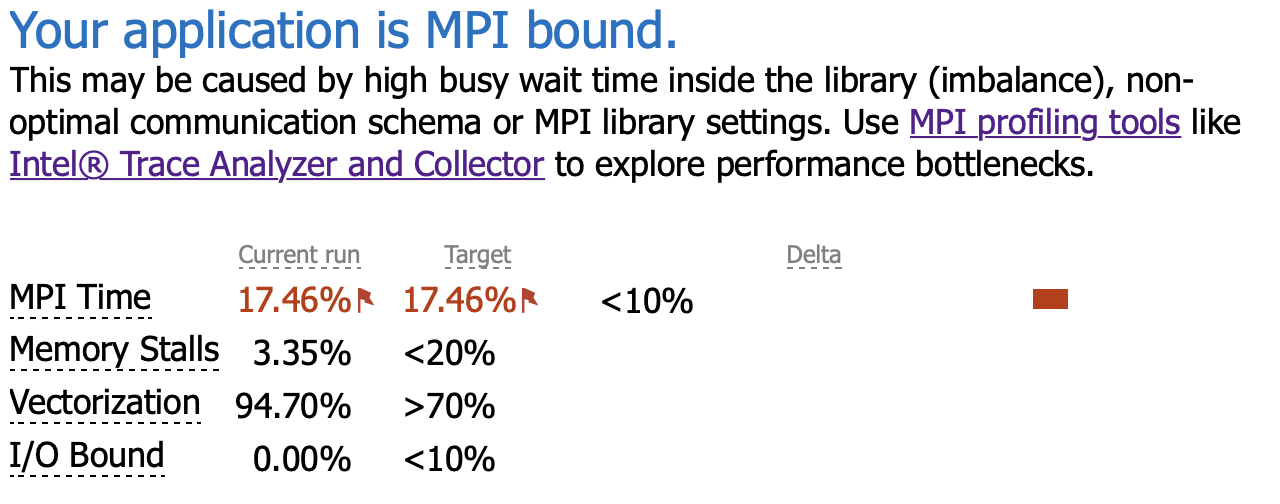
\includegraphics[width=1.\linewidth]{Images/VTUNE_APS/original.png}
		\caption{Unoptimised NCU implementation. Total compute time was $783.33$s.}
        \label{fig:aps_unopt_ncu}
    \end{subfigure}\\
    \begin{subfigure}{.8\linewidth}
        \centering
        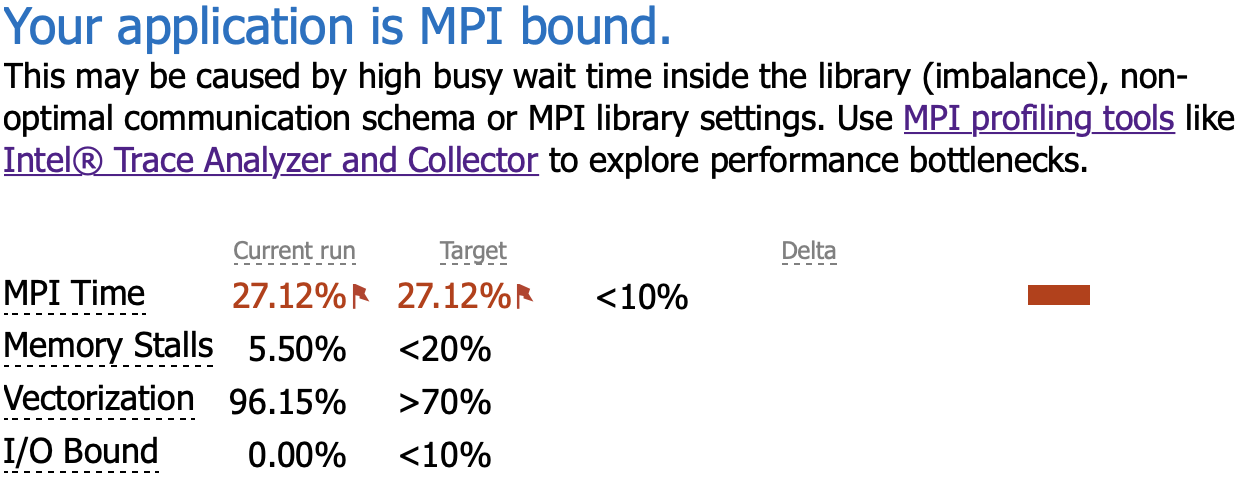
\includegraphics[width=1.\linewidth]{Images/VTUNE_APS/ncu_opt.png}
		\caption{Optimised NCU implementation. Total compute time was $449.91$s.}
        \label{fig:aps_opt_ncu}
    \end{subfigure}
    \caption{APS summaries for both unoptimised and optimised NCU operations for the application. Note, the reduction in the runtime of the the optimised routine in Figure~\ref{fig:aps_opt_ncu}.}
        \label{fig:aps}
\end{figure}

In both cases, it reported that the application is MPI bound and recommended a more detailed profiling analysis using the Intel\textregistered Trace Analyzer \& Collector.

Although the percentage of time spent in MPI routines increased after applying the optimisation, the runtime has almost halved. The time spent in vectorised routines increases. To gain a better understanding of the behaviour, further profiling was conducted.


\subsection{Intel\textregistered Trace Analyzer \& Collector (ITAC)}
\label{sec:Intel_ITAC}
Upon the recommendation of the the Intel\textregistered VTune APS, the ITAC tool was run for both versions of the application. It collects and analyses the inter-process communication including between nodes. 

\subsubsection{Serial versus Parallel Comparison}
Figure~\ref{fig:itac_pie} shows the percentage of total run-time spent in serial, MPI, and threaded regions. The percentage of time spent on serial regions decreases by $1.2\%$, but MPI regions increase by $6.2\%$ after the \textit{nCU} optimisations. 

\begin{figure}[H]%[!ht]
    \centering
    \begin{subfigure}{1.\linewidth}
        \centering
        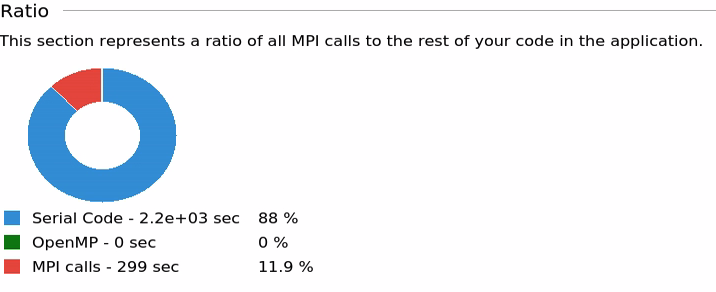
\includegraphics[width=1.\linewidth]{Images/MPI_Serial_Pie/orig_pie.png}
		\caption{Unoptimised NCU implementation.}
        \label{fig:itac_pie_unopt_ncu}
    \end{subfigure}\\
    \begin{subfigure}{1.\linewidth}
        \centering
        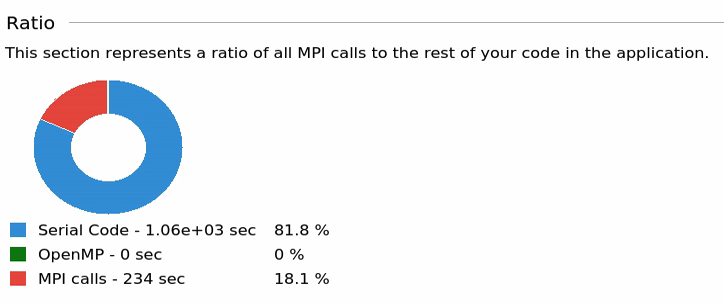
\includegraphics[width=1.\linewidth]{Images/MPI_Serial_Pie/ncu_pie.png}
		\caption{Optimised NCU implementation.}
        \label{fig:itac_pie_opt_ncu}
    \end{subfigure}
    \caption{ITAC breakdown of time spent in serial, MPI and OpenMP sections     for both unoptimised and optimised NCU operations for the application.}
        \label{fig:itac_pie}
\end{figure}

Taking the significant reduction in runtime by almost $50\%$ into account after the optimisations, it is clear that the time spent in both MPI and serial regions have decreased significantly. Now MPI routines are taking up a larger percentage of the runtime.

\subsubsection{Overview of MPI Routines}
\label{sec:overview_MPI_routines}
The breakdown of the comparison between each of the most active MPI routines are visible in Figure~\ref{fig:itac_mpi_bar}. \textit{MPI\_Sendrecv} is responsible for the majority of MPI overhead. \textit{MPI\_Comm\_size} and \textit{MPI\_Comm\_rank} respectively contribute a lot less but still relatively significantly to the MPI overhead. This did not change after the \textit{nCU} optimisations were applied. The runtime for each of these routines decreased but their percentage contribution to the runtime increased.

\begin{figure}[!ht]
    \centering
    \begin{subfigure}{1.\linewidth}
        \centering
        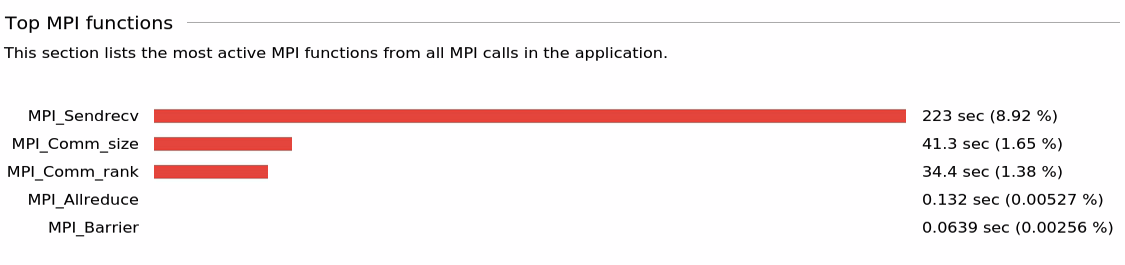
\includegraphics[width=1.\linewidth]{Images/MPI_Comms_Bar/orig_comms_bar.png}
		\caption{Unoptimised NCU implementation.}
        \label{fig:itac_mpi_bar_unopt_ncu}
    \end{subfigure}\\
    \begin{subfigure}{1.\linewidth}
        \centering
        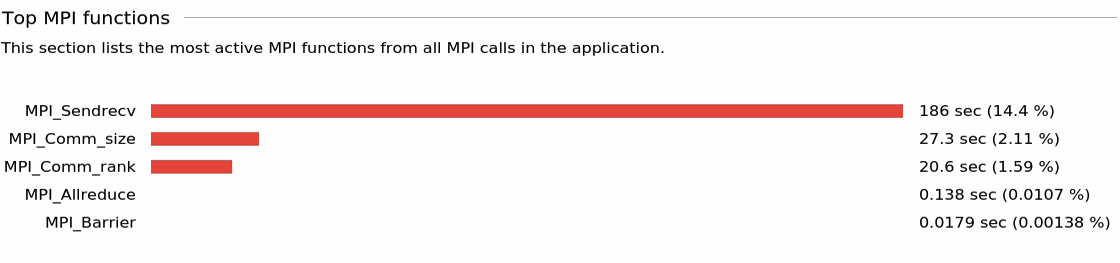
\includegraphics[width=1.\linewidth]{Images/MPI_Comms_Bar/ncu_comms_bar.png}
		\caption{Optimised NCU implementation.}
        \label{fig:itac_mpi_bar_opt_ncu}
    \end{subfigure}
    \caption{ITAC summary breakdown of time spent in different MPI routines for both unoptimised and optimised NCU operations for the application.}
        \label{fig:itac_mpi_bar}
\end{figure}

\subsubsection{Event and Quantitative Timelines}
An event timeline and quantitative timeline can be seen in Figure~\ref{fig:itac_comms_bar} for approximately a single iteration of both the unoptimised and optimised versions of the application. First, note that Figure~\ref{fig:itac_mpi_comms_unopt_ncu} is not shown in as fine time resolution as Figure~\ref{fig:itac_mpi_comms_opt_ncu}, so they are not directly quantitatively comparable. The event timeline depicts the MPI communication between each of the four processes. The quantitative timeline more clearly depicts which processes where involved in the communications and the duration of the communications. 

In Figure~\ref{fig:itac_mpi_comms_unopt_ncu}, majority of the MPI communications are across all of the processes. In contrast, in Figure~\ref{fig:itac_mpi_comms_opt_ncu} the MPI communication is rarely across all processes, instead using point-to-point communications. Comparing these two figures, the optimised \textit{nCU} version has in general less expensive MPI communication routines across all of the processes, and thus there is less MPI overhead.

\begin{figure}[H]%[!ht]
    \centering
    \begin{subfigure}{1.\linewidth}
        \centering
        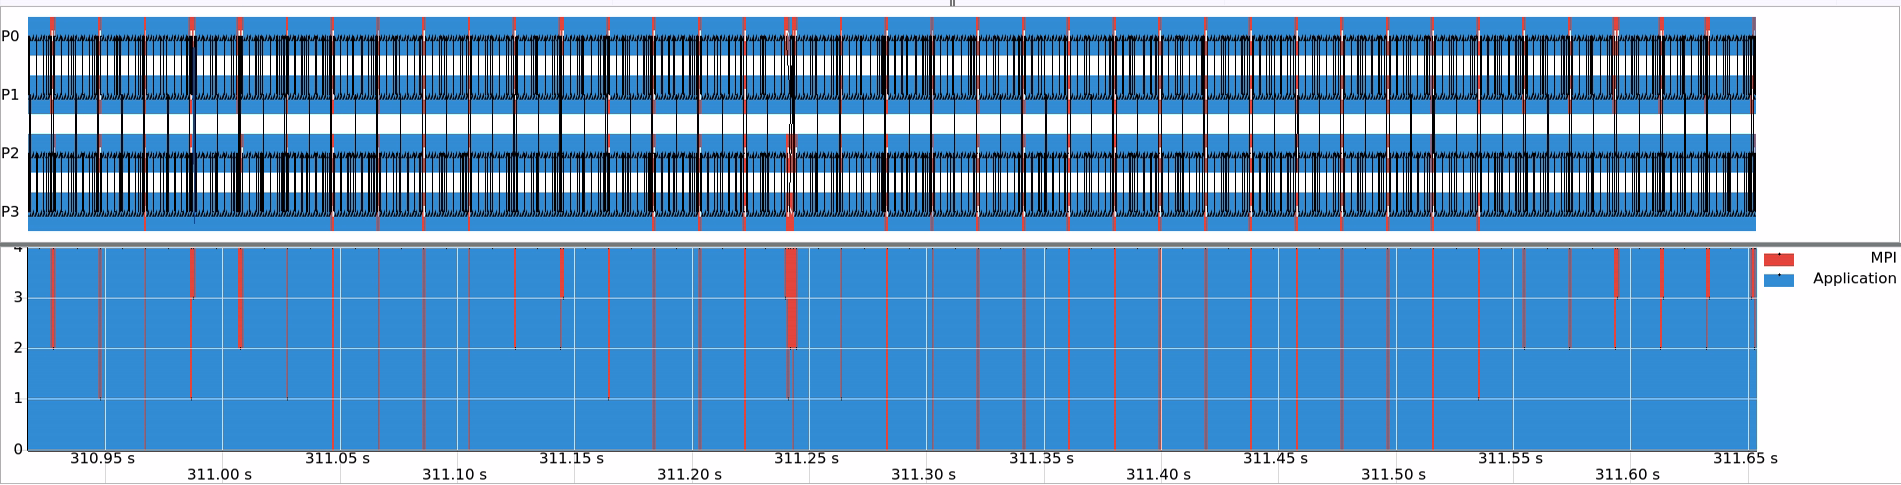
\includegraphics[width=1.\linewidth]{Images/App_iteration/orig_single_iteration.png}
		\caption{Unoptimised NCU implementation.}
        \label{fig:itac_mpi_comms_unopt_ncu}
    \end{subfigure}\\
    \begin{subfigure}{1.\linewidth}
        \centering
        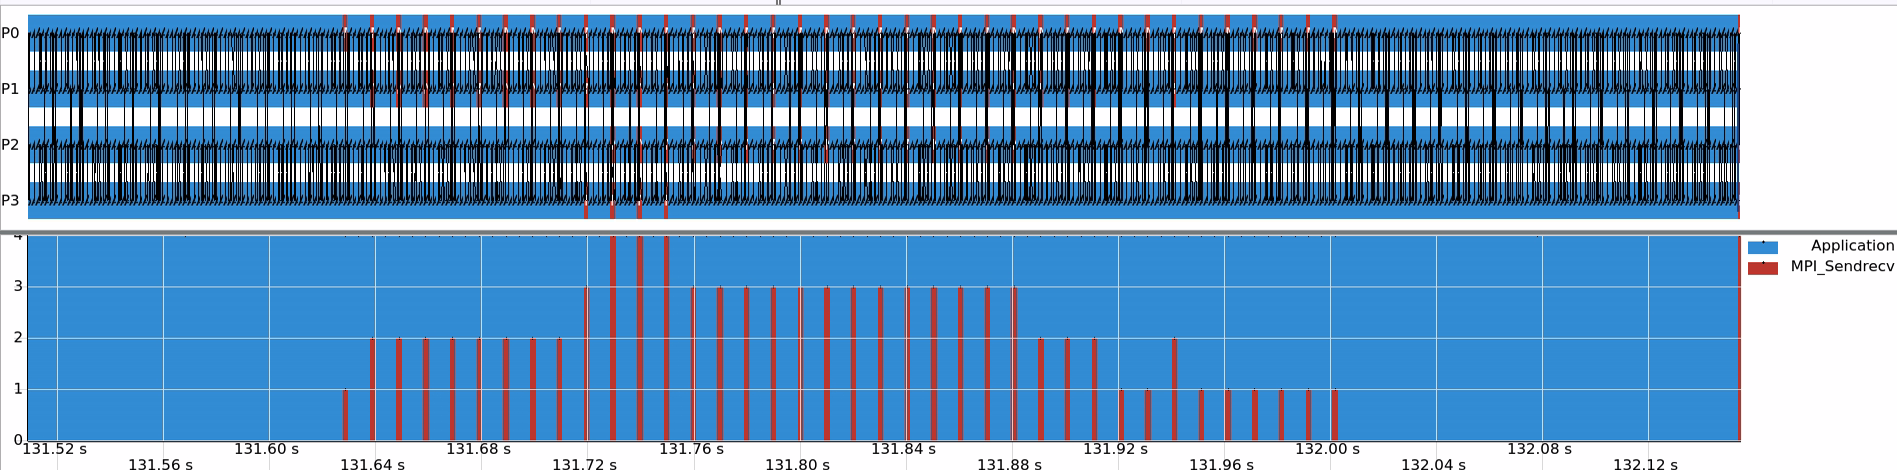
\includegraphics[width=1.\linewidth]{Images/App_iteration/ncu_single_iteration.png}
		\caption{Optimised NCU implementation.}
        \label{fig:itac_mpi_comms_opt_ncu}
    \end{subfigure}
    \caption{ITAC event (top of each subfigure) and quantitative (bottom of each subfigure) timelines for approximately a single iteration of both the unoptimised and optimised \textit{nCU} operations for the application.}
        \label{fig:itac_comms_bar}
\end{figure}

\subsubsection{MPI Call Counts}
Figure~\ref{fig:itac_counts_unopt_ncu} and~\ref{fig:itac_counts_opt_ncu} detail the call counts and corresponding execution times for the unoptimised and optimised \textit{nCU} routines respectively. The lists are ordered by decreasing call counts. \textit{MPI\_Comm\_size} is called approximately $278\times10^6$ times and $190\times10^6$ for the unoptimised and optimised routines respectively. Similarly, $142\times10^6$ and $98\times10^6$ for \textit{MPI\_Comm\_rank}, $12\times10^6$ and $13\times10^6$ for \textit{MPI\_Sendrecv}, $14\times10^3$ and $2\times10^3$ for \textit{MPI\_Barrier}, and $12\times10^3$ and $0$ for \textit{MPI\_Bcast}. All of the other call counts remained approximately the same.

From Section~\ref{sec:overview_MPI_routines}, \textit{MPI\_Comm\_size} consists of $1-2\%$ of runtime, and \textit{MPI\_Comm\_rank} $1.3-1.6\%$. From Figure~\ref{fig:itac_counts}, they are responsible for a very large number of MPI calls, being called more than any other MPI routine. After applying the \textit{nCU} optimisations, their call counts are reduced considerably, but still account for majority of MPI calls. These two routines should ideally only be called at the very beginning of the application when the MPI environment is initialised. However, Intel\textregistered-QS calls them in its quantum gate calls. Thus, if Intel\textregistered-QS has these calls removed  from its gate calls and instead stores these calls' initial values as constant values, a small but significant overhead will disappear. Also note, these calls only increase as the problem size increases, scaling with the gate depth and hence problem size.

The number of \textit{MPI\_Send\_recv} calls increased by approximately $1\times10^6$ after the optimisations. However, the number of \textit{MPI\_Bcast} was reduced from $12\times10^6$ to zero. The extra \textit{MPI\_Send\_recv} was due to the re-implementation of the \textit{nCU} routine, which also got rid of the need of \textit{MPI\_Bcast}'s. The latter of the two can be considered to be more expensive since it is a group communication rather than just involving two processes (also taking the quantity of the reduction into account), even though \textit{MPI\_Send\_recv} is blocking and \textit{MPI\_Bcast} is not. This explains a portion of the performance increase.

There is also a significant reduction in the number of expensive \textit{MPI\_Barrier} calls after the optimisations. This is a significant improvement.

\begin{figure}[H]%[!ht]
    \centering
    \begin{subfigure}{1.\linewidth}
        \centering
        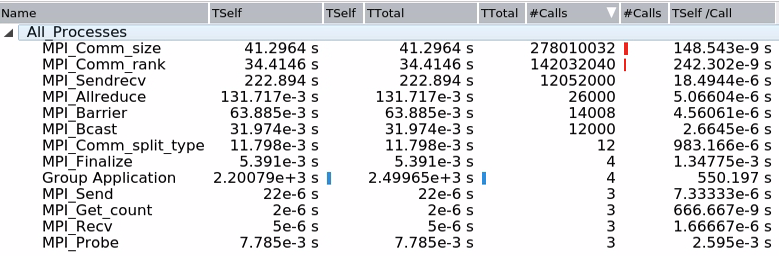
\includegraphics[width=1.\linewidth]{Images/MPI_message_counts/orig_message_counts.png}
		\caption{Unoptimised NCU implementation.}
        \label{fig:itac_counts_unopt_ncu}
    \end{subfigure}\\
    \begin{subfigure}{1.\linewidth}
        \centering
        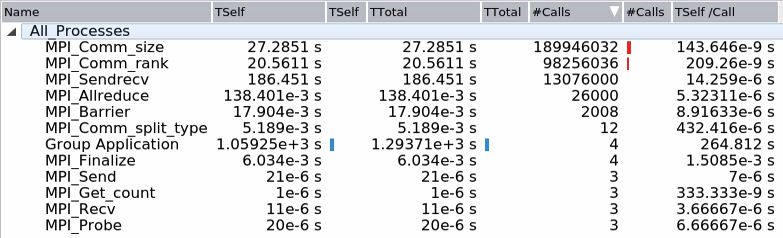
\includegraphics[width=1.\linewidth]{Images/MPI_message_counts/ncu_message_counts.png}
		\caption{Optimised NCU implementation.}
        \label{fig:itac_counts_opt_ncu}
    \end{subfigure}
    \caption{ITAC MPI message counts for both the unoptimised and optimised NCU operations for the application.}
        \label{fig:itac_counts}
\end{figure}

\subsection{Intel\textregistered VTUNE Amplifier}
Intel\textregistered VTUNE Amplifier was used to profile the behaviour of the application on a single node, taking more detailed measurements into consideration including hardware metrics. This allows for a more detailed analysis of the applications behaviour and can indicate individual functions and regions of code that contribute to overhead.

A summary of which source files contribute to the majority of CPU utilisation occurred is shown in Figure~\ref{fig:vtume_amplxe_summary}. The first seven of these source files are from the Intel\textregistered-QS. The first three of these account for the majority of CPU utilization. The biggest contributor is the \textit{highperfkernel.cpp} source file. Upon switching to a view which was grouped by the function call stack, the same observations were made.

The \textit{apply\_ctrl2qubitgate.cpp} source file and the \textit{ncu.hpp} header file were identified as the biggest contributors from the QNLP library. The first of these calls routines from the Intel\textregistered-QS library directly, so cannot be optimised further. Further optimisations are possible for the \textit{nCU} implementation, however due to time constraints, will be put on hold.

\begin{figure}[H]%[!ht]
    \centering
    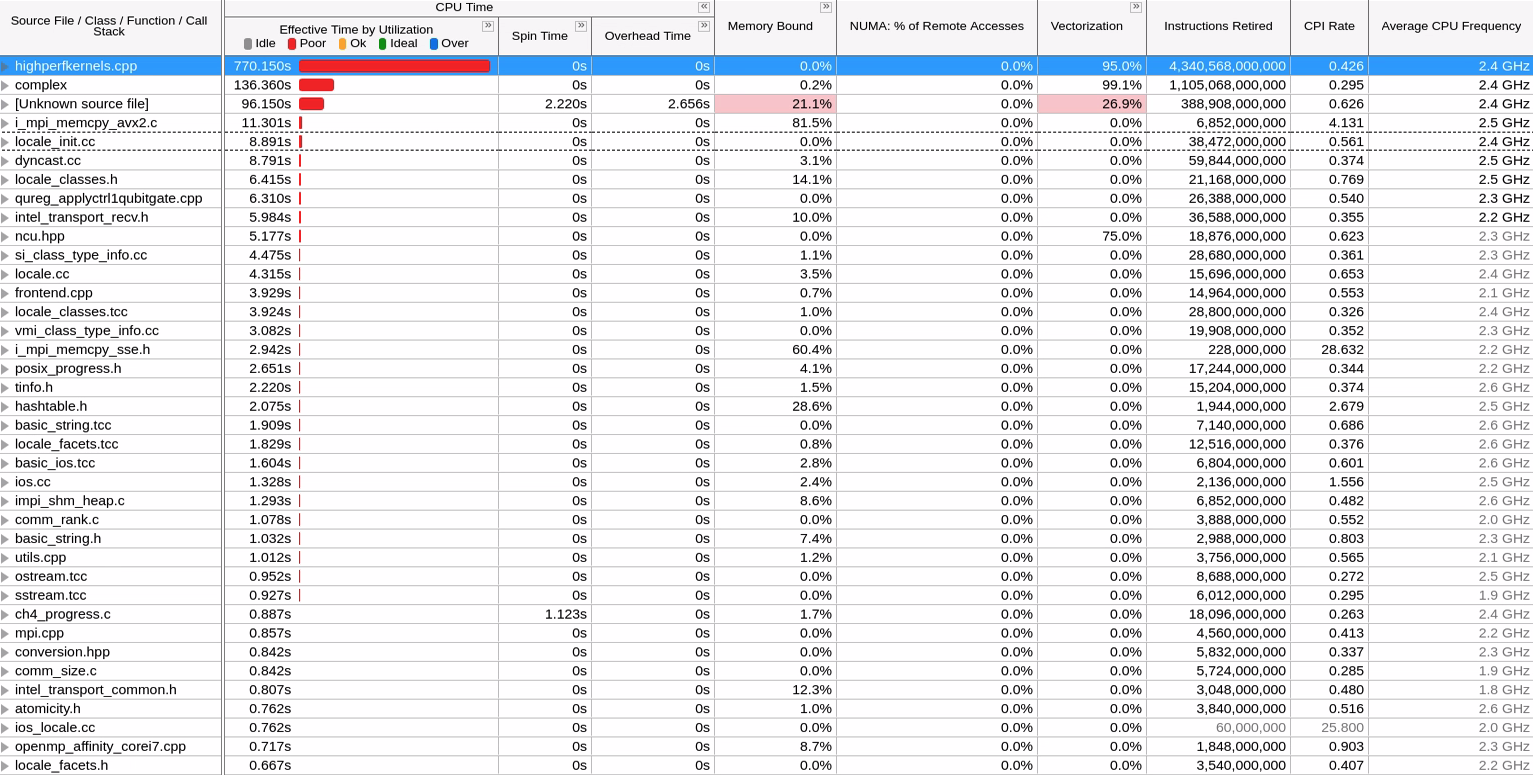
\includegraphics[width=1.\linewidth]{Images/VTUNE_Amplxe/vtune_amplxe_summary.png}
	\caption{Summary of main contributors of CPU utilization using Intel\textregistered VTUNE Amplifier.}
    \label{fig:vtume_amplxe_summary}
\end{figure}

\subsection{Profiling Conclusions}

The increase in the percentage of the MPI routines after the \textit{nCU} optimisations were applied is an expected outcome. The optimisations reduced the amount of quantum gate calls significantly, including multi-qubit controlled gates. This led to less MPI communications being executed, and also to less regions of serial code being executed. However, the other serial parts of the application remained unaffected by these optimisations, thus the percentage of time spent in MPI routines increased despite the runtime decreasing.

The main bottleneck originated from the \textit{nCU} gate calls. The underlying simulator only has a number of more fundamental gate operations available, consisting of single qubit, and one and two qubit controlled gate operations. The \textit{nCU} gate is an $n$ qubit controlled unitary operation. To implement it, it is decomposed into a series of the fundamental operations previously mentioned. These operations often involve MPI communication to execute successfully. As $n$ becomes larger, the number of gate operations that comprise the \textit{nCU} gate call grows very quickly. This \textit{nCU} gate call is used a number of times in the encoding steps of the algorithm. Thus, one of the reasons for the MPI bound nature of the application is apparent. After applying the optimisations, this routine is still a major contributor to the application's overhead. This is because although the circuit depth has been significantly decreased by the optimisations, it is still very large.

Removing the \textit{MPI\_Comm\_size} and \textit{MPI\_Comm\_rank} calls from the gate operations in the Intel\textregistered-QS would give the application (and similar applications) a small but consistent performance increase.

After using the Intel{\textregistered}VTUNE Amplifier, it is evident that the \textit{highperfkernel.cpp} source file from the Intel\textregistered-QS is the biggest contributor to the overhead caused by poor CPU utilization. It would require further and more detailed profiling analysis to identify whether any performance gain can be made, or if it is already optimal. However, making changes to the Intel\textregistered-QS is beyond the scope of this project.

It is noted that further optimisations could be made to the \textit{nCU} implementation which would give a slight performance improvement by reducing the number of gate calls. If time permits, this will be looked into in further detail.
